\chapter{Anhang}
\subsubsection{Gesamtschaltbild}
\begin{figure}[H]
\centering
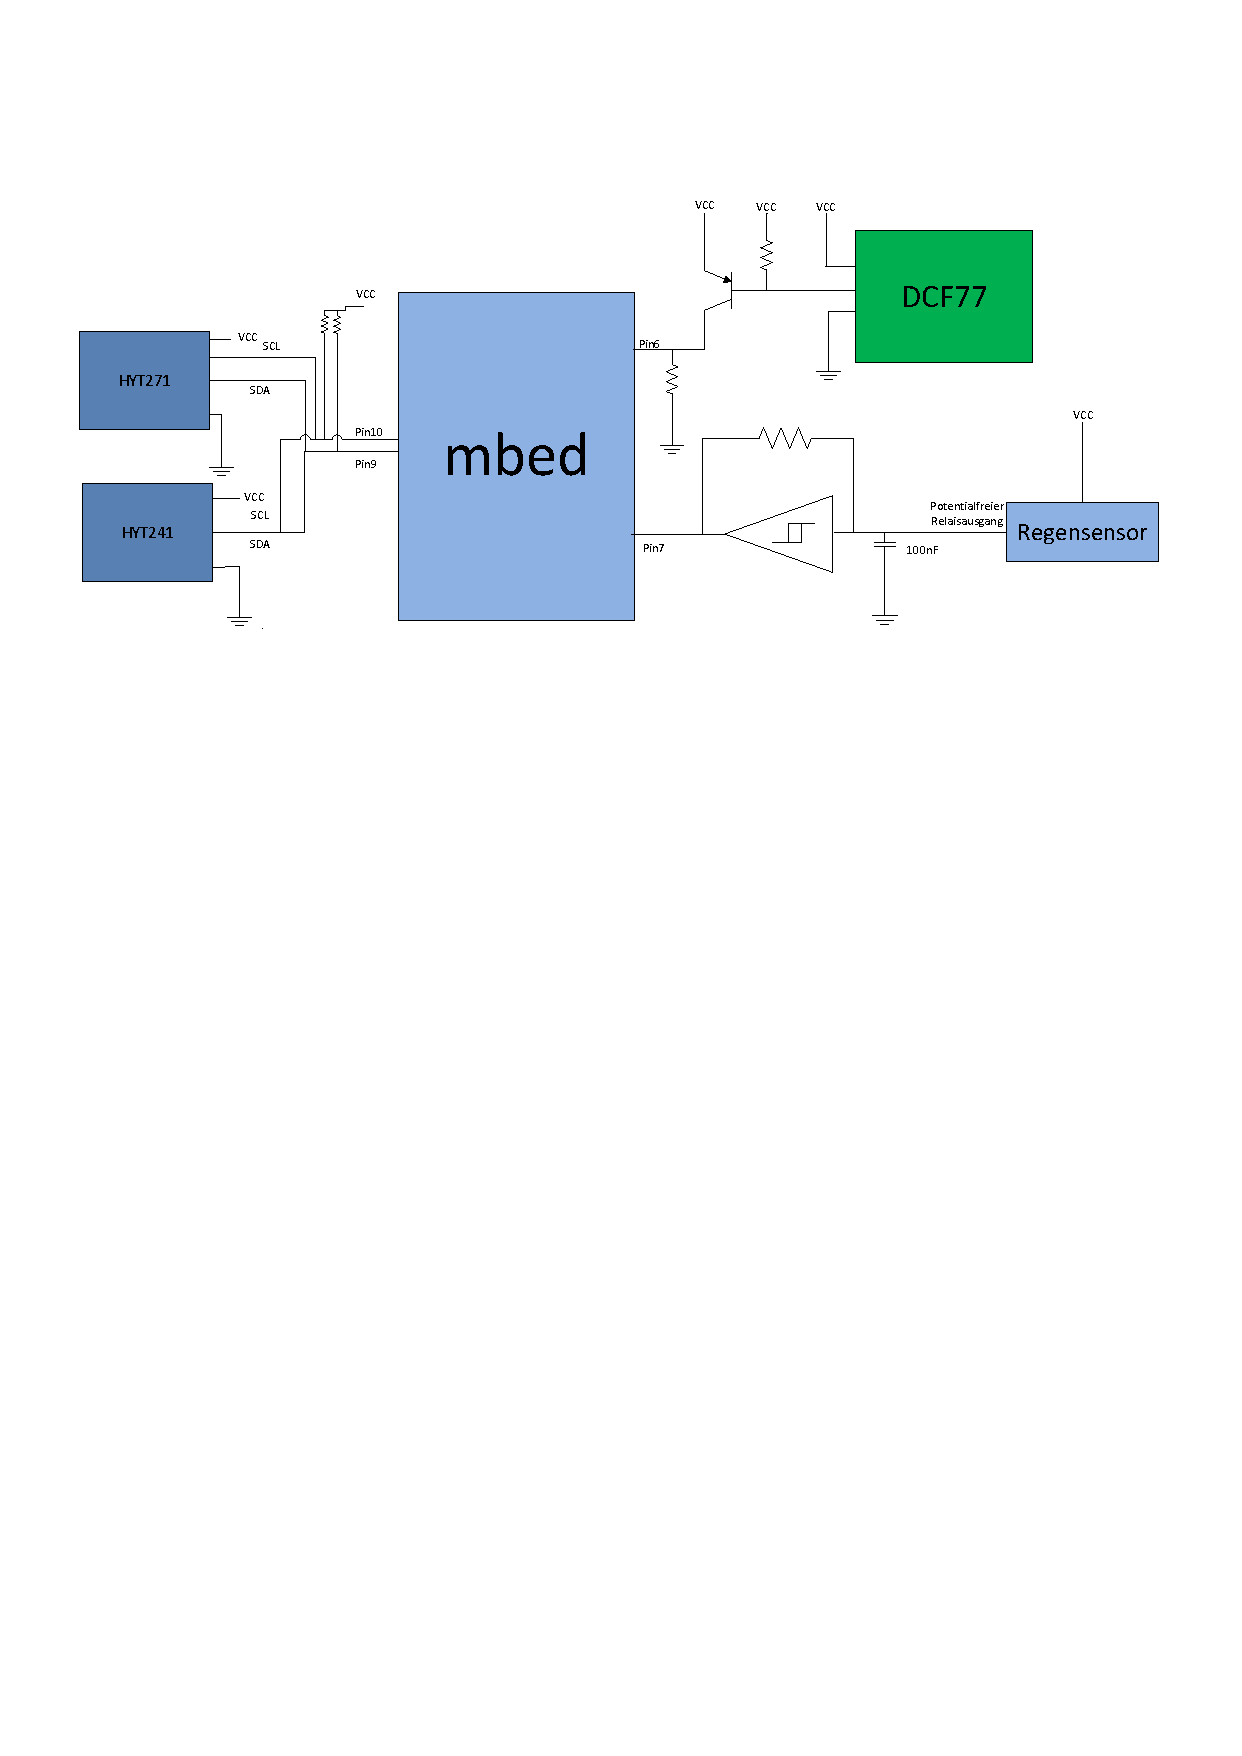
\includegraphics[width=\textwidth]{./Schaltplaene/Gesamt-Schaltung}
\caption{Gesamtschaltung des Projektes}
\label{fig:Gesamt-Schaltung}
\end{figure}
\subsubsection{Funktionsübersicht des Projektes}
\underline{\textbf{DCF77}}
\begin{description}
\item[timeDCF77* getTime()] Gibt die aktuell empfangene Zeit zurück.
\item[bool recieveTime()] Startet den Empfangsvorgang des DCF77 Empfängers.
\item[void setRTCClock()] Setzt die Real-Time-Clock des mbed Mikrocontrollers.
\item[void changeDebugState()] Lässt LEDs blinken wenn das DCF77 Signal empfangen wird. bzw. schaltet es wieder aus.
\end{description}
\underline{\textbf{HYT2x1}}
\begin{description}
\item[float getTemp()] Gibt die Aktuell empfangene Temperatur zurück.
\item[float getHumid()] Gibt die Aktuell empfangene relative Luftfeuchtigkeit zurück.
\item[bool update()] Startet einen neuen Messvorgang.
\item[bool setAdress()] Startet die Routine zum ändern der Adresse des HYT2x1. 
\end{description}
\underline{\textbf{Regensensor}}
\begin{description}
\item[getRain()] Gibt des aktuellen Regenstatus zurück.
\end{description}
\underline{\textbf{Logging}}
\begin{description}
\item[bool log(char Log[])] Schreibt den Parameter in den RAM des mbed Mikrocontrollers.
\end{description}

\subsubsection{DCF77 Empfangstabelle}
	\begin{table}[H]
		\begin{tabular}{ |l|p{7cm}| p{5cm}| }
			\hline \textbf{Bit} & \textbf{Bedeutung} & \textbf{Anmerkung} \\ 
			\hline 0 & Start einer neuen Minute & Ist immer 0 \\ 
			\hline 1-14 & Wetterinformationen der Firma MeteoTime und Katastrophenschutzinformationen & \\
			\hline 15 & Rufbit & \\
			\hline 16 & MEZ/MESZ Umstellung & 1: Am Ende dieser Stunde wird MEZ/MESZ umgestellt \\
			\hline 17 & MEZ Information & 0: MEZ, 1: MESZ \\
			\hline 18 & MEZ Information & 0: MESZ, 1: MEZ \\
			\hline 19 & Schaltsekunde & 1: Am Ende dieser Stunde wird eine Schaltsekunde eingefügt \\
			\hline 20 & Beginn der Zeitinformationen & Ist immer 1 \\
			\hline 21-27 & Minuten & \\
			\hline 28 & Parität Minuten & \\
			\hline 29-34 & Stunden & \\
			\hline 28 & Parität Stunden & \\
			\hline 36-41 & Kalendertag & \\
			\hline 42-44 & Wochentag & \\
			\hline 45-49 & Montsnummer & \\
			\hline 50-57 & Jahr & \\
			\hline 58 & Parität Datum & \\
			\hline 
		\end{tabular}
		\caption[DCF77 - Frameaufbau]{DCF77 - Frameaufbau, Quelle: \cite{DCF77Wiki}}
		\label{table:DCF77Frame}
	\end{table}

